\chapter{Unit testen met JUnit}

De software die we ontwikkelen moet kwaliteitsvol zijn. Maar hoe kunnen we er nu voor zorgen dat we het aantal bugs in onze code zo laag mogelijk houden? E\'en van de strategie\"en om de kwaliteit van software te waarborgen is testen. Testen is een heel belangrijk aspect van softwareontwikkeling waar je ongetwijfeld nog heel veel over gaat leren. 

Als ontwikkelaar zorg je er altijd voor dat wanneer je de gevraagde functionalteit implementeert, je ook de nodige unit testen schrijft om de kwaliteit van je code te garanderen. Wanneer je unit testen schrijft, ga je alle methoden van je klasse testen. Een methode van een klasse is dus de ``unit'' die we gaan testen.
We gaan automatische testen schrijven. Dit betekent dat iedere keer dat de code wordt aangepast of uitgebreid de testen eenvoudig opnieuw kunnen worden uitgevoerd. Op die manier gaan de fouten die ontstaan tijdens de verdere ontwikkeling van de software snel ontdekt worden. Bedenk ook dat een fout, onduidelijkheid of bug die vroeg in het ontwikkelproces wordt aangepakt, maar een kleine impact heeft (ook financieel) ten opzicht van problemen die later pas opduiken.

Als je unit testen schrijft hoef je geen schrik te hebben om achteraf code aan te passen en te verbeteren. Omdat je beschikt over unit testen kan je rustig aan je code sleutelen. Het proces om code te verbeteren en hierdoor de leesbaarheid en onderhoudbaarheid van de code te verhogen noemen we \textbf{refactoren}. 

\section{JUnit}

In Java gebruiken we het framework JUnit5 om onze unit testen te schrijven.
JUnit5 is opgedeeld in 3 sub-projecten:  Jupiter, Vintage en Platform. JUnit Jupiter is het  sub-project dat wij gebruiken om onze testen te schrijven en voorziet de engine om deze testen uit te voeren.

De dependency  spring-boot-starter-test wordt altijd toegevoegd aan een Spring Boot project. 

\begin{verbatim}
<dependency>
	<groupId>org.springframework.boot</groupId>
	<artifactId>spring-boot-starter-test</artifactId>
	<scope>test</scope>
</dependency>
\end{verbatim}

De scope test is belangrijk en duidt erop dat de depencendy niet nodig is voor het normale gebruik van de toepassing.  De dependency is enkel nodig voor het compileren en uitvoeren van de testen.



\section{De klasse House}

We gaan nu unit testen schrijven voor onderstaande klasse House. 

\begin{lstlisting}
package be.pxl.domain;

public class House {
    private static final double BASE_PRICE = 2356.75;
 	private final String code;
    private String description;
    private int area;
    private String city;
    private Status status;
    private EPCScore epcScore;

    public House(String code, String description, int area, EPCScore epcScore) {
        this.code = code;
        this.description = description;
        this.area = area;
        this.epcScore = epcScore;
        this.status = Status.FOR_SALE;
    }

    public String getDescription() {
        return description;
    }

    public void setDescription(String description) {
        this.description = description;
    }

    public void setEpcScore(EPCScore epcScore) {
        this.epcScore = epcScore;
    }

    public String getCode() {
        return code;
    }

    public int getArea() {
        return area;
    }

    public void setArea(int area) {
        this.area = area;
    }

    public String getCity() {
        return city;
    }

    public Status getStatus() {
        return status;
    }

    public EPCScore getEpcScore() {
        return epcScore;
    }

    public void setCity(String city) {
        this.city = city;
    }

    public void markAsSold() {
        if (Status.FOR_SALE == status) {
            status = Status.SOLD;
        } else {
            throw new IllegalStateException("House is already marked as sold.");
        }
    }

    public double getPrice() {
        double price = area * BASE_PRICE * epcScore.getPercentage();
        if ("Hasselt".equals(city) || "Genk".equals(city)) {
            price *= 1.25;
        }
        return price;
    }
}

\end{lstlisting}

\begin{lstlisting}
package be.pxl.domain;

public enum EPCScore {
	A_PLUS(1.5),
	A(1.2),
	B(1),
	C(0.98),
	D(0.90),
	E(0.80),
	F(0.75);

	private double percentage;

	EPCScore(double percentage) {
		this.percentage = percentage;
	}

	public double getPercentage() {
		return percentage;
	}
}
\end{lstlisting}


\section{Klasse met de unit testen}

In een Spring Boot-project met Maven als build tool worden de klassen met unit testen in een specifieke mapstructuur geplaatst. 

De conventie is om testklassen in de map \textbf{src/test/java} te plaatsen.  De testklassen moeten zich in deze map bevinden, georganiseerd in dezelfde packages als de bronklassen.

Bijvoorbeeld, als de bronklassen zich in het package be.pxl.myapp bevinden, moeten de testklassen zich bevinden in de folder src/test/java/be/pxl/myapp.

Het is handig om de testklassen namen te geven die eindigen op \textbf{Test} om duidelijk aan te geven dat het om testen gaat. De testen voor de klasse MyService noem je dus MyServiceTest.

Maak nu de klasse HouseTest in het package be.pxl.domain in de folder src/test/java.

\section{Unit test voor de constructor}

We gaan starten met een test te schrijven om de constructor te testen.  We controleren of alle velden correct worden ingevuld als we de constructor hebben aangeroepen.  Verder controleren we ook dat de city geen waarde krijgt en de initi\"ele waarde voor de status van het huis FOR\_SALE is.

\begin{lstlisting}
package be.pxl.domain;

import org.junit.jupiter.api.BeforeEach;
import org.junit.jupiter.api.Test;
import static org.junit.jupiter.api.Assertions.*;

public class HouseTest {
    
    @Test
    public void testConstructor() {
        House house = new House("XYZ789", "2-bedroom apartment", 100, EPCScore.B);

        assertEquals("XYZ789", house.getCode());
        assertEquals("2-bedroom apartment", house.getDescription());
        assertEquals(100, house.getArea());
        assertEquals(EPCScore.B, house.getEpcScore());
        assertEquals(Status.FOR_SALE, house.getStatus());
        assertNull(house.getCity()); // City is not set initially
    }
}
\end{lstlisting}


We voegen bij een methode in de testklasse de annotatie @Test toe zodat de test herkend wordt en uitgevoerd kan worden. 

Wanneer je de testklasse HouseTest uitvoert kunnen er 3 mogelijke scenario's plaatsvinden. Ofwel slaagt de test, ofwel faalt \'e\'en van de beweringen (asserts) ofwel loopt er iets onverwachts fout. In het eerste geval krijgt de test een groene kleurcode, in het tweede scenario een oranje en in het laatste scenario een rode.

\begin{figure}[H]
  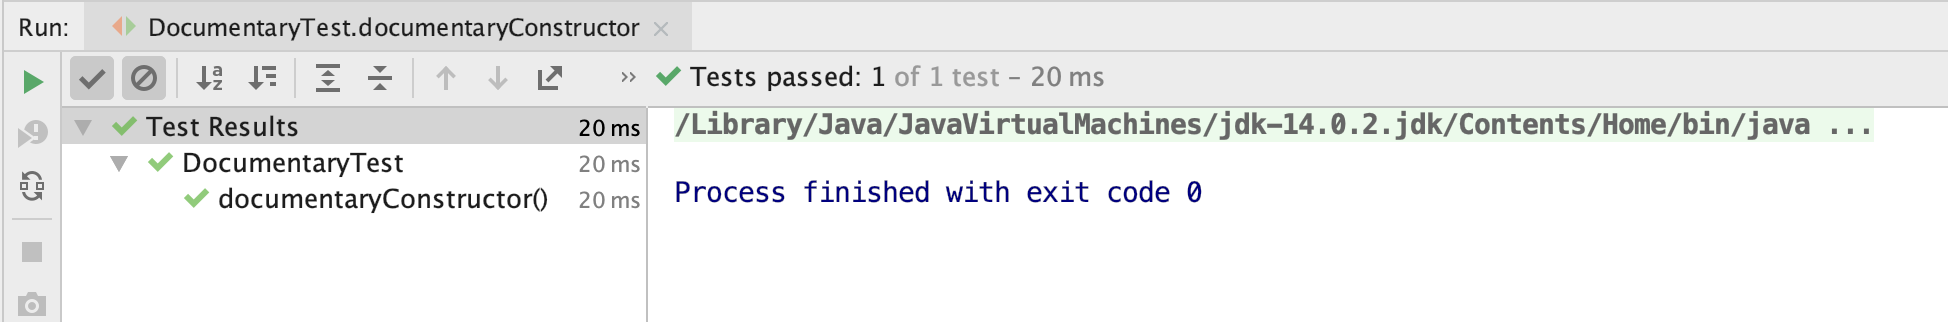
\includegraphics[width=\linewidth]{images/chapter-junit/junit_test_passed.png}
  \caption{Geslaagde JUnit5 test}
  \label{fig:test_passed}
\end{figure}

\begin{figure}[H]
  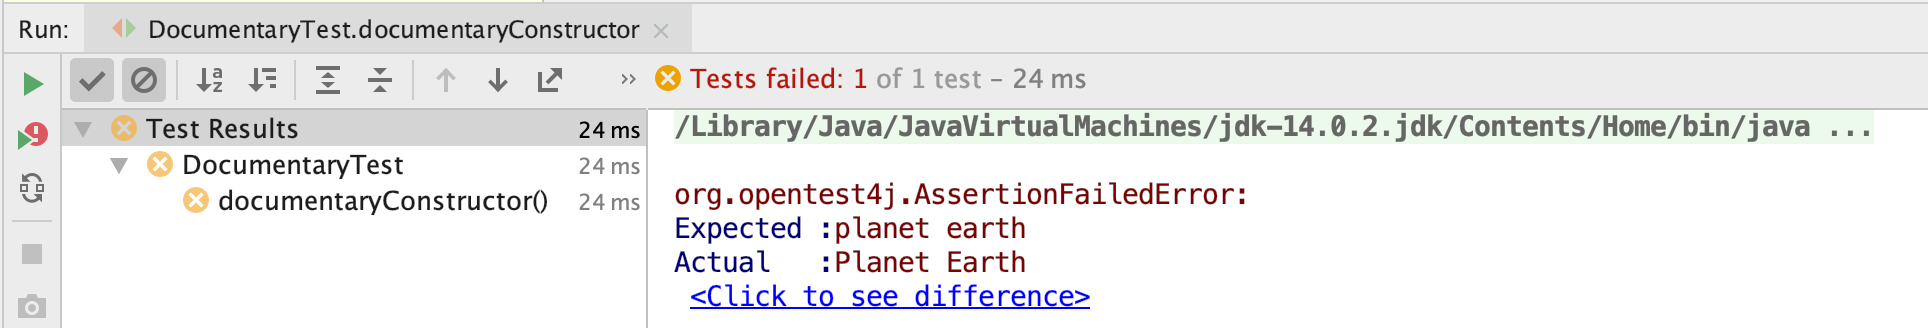
\includegraphics[width=\linewidth]{images/chapter-junit/junit_test_failed.png}
  \caption{Gefaalde JUnit5 test}
  \label{fig:test_failed}
\end{figure}

Hier is een overzicht van enkele handige static methoden uit de klasse org.junit.jupiter.api.Assertions. 

\begin{table}[h!]
\centering
\begin{tabularx}{\textwidth}{| l | X |}
 \hline
 Methode & Betekenis\\ 
 \hline\hline
assertEquals() & Evalueert de gelijkheid van 2 waarden. De test slaagt als beide
waarden gelijk (equal) zijn.\\
\hline
assertFalse() & Evaluatie van een booleaanse uitdrukking. De test slaagt indien
de uitdrukking false is.\\
\hline
assertTrue() & Evaluatie van een booleaanse uitdrukking. De test slaagt indien
de uitdrukking true is.\\
\hline
assertNotNull( ) & Vergelijkt een object referentie met null. De test slaagt indien de
object referentie niet null is.\\
\hline
assertSame( ) & Vergelijkt het geheugenadres van twee object referenties
(gebruik maken van == operator). De test slaagt indien beide
object referenties naar hetzelfde object verwijzen.\\
\hline
fail() & Zorgt ervoor dat de test zal falen.\\
 \hline
\end{tabularx}
\caption{Static methoden uit de klasse org.junit.jupiter.api.Assertions}
\label{table:assertions}
\end{table}

\section{Unit test voor een setter}

Een unit test wordt steeds opgebouwd volgens het 3A patroon: Arrange, Act en Assert.
In iedere test herken je steeds deze 3 bouwstenen. 

Het ``arrange''-gedeelte is waar het object dat getest moet worden en alle andere objecten - die nodig zijn om de test goed uit te voeren - worden aangemaakt. 
Het ``act''-gedeelte is waar we de methode die we willen testen aanroepen. Als de methode een returnwaarde heeft ken je dit toe aan een variabele.

Het ``assert''-gedeelte geeft je de mogelijkheid om beweringen over het resultaat te verifi\"eren.

\global\csname @topnum\endcsname 0

Laten we de methode setCity() testen.  We controleren dat een object, na het aanroepen van de methode setCity met een gekozen parameter, correct werd aangepast.

\begin{lstlisting}
import org.junit.jupiter.api.BeforeEach;
import org.junit.jupiter.api.Test;
import static org.junit.jupiter.api.Assertions.*;

public class HouseTest {
  
    @Test
    public void testSetCity() {
        House house = new House("ABC123", "3-bedroom house", 150, EPCScore.GOOD);
    	   house.setCity("Dilsen-Stokkem");
        assertEquals("Dilsen-Stokkem", house.getCity());
    }
}
\end{lstlisting}

\clearpage

\section{@BeforeEach}

De annotatie @BeforeEach wordt gebruikt om een methode aan te duiden die vóór elke testmethode in de testklasse wordt uitgevoerd. Deze methode wordt gebruikt voor herhaalbare initialisatiecode die nodig is voor elke (of bijna elke) testmethode.
Het vermindert duplicatie van code door gedeelde initialisatie te centraliseren.
Deze methode heeft geen parameters en geen returnwaarde.

\begin{oefening}
Voeg een test toe voor iedere setter in de klasse House.
\end{oefening}

\section{Unit test voor een berekende waarde}

In de klasse House vind je de methode getPrice() terug. Deze methode bevat een berekening die we uiteraard willen testen.

Bedenk welke scenario's er kunnen voorkomen en zorg dat je een test schrijft voor elk scenario.

\begin{lstlisting}
import org.junit.jupiter.api.BeforeEach;
import org.junit.jupiter.api.Test;
import static org.junit.jupiter.api.Assertions.*;

public class HouseTest {
    private House house;

    @BeforeEach
    public void setUp() {
        house = new House("ABC123", "3-bedroom house", 250, EPCScore.B);
    }
    

    @Test
    public void testGetPrice() {
        house.setArea(150);
        double expectedPrice = 150 *House.BASE_PRICE * EPCScore.B.getPercentage();
        assertEquals(expectedPrice, house.getPrice(), 0.001);
    }
    
    @Test
    public void testGetPriceWithCity() {
    	    house.setArea(150);
        house.setCity("Hasselt");
        
        double expectedPrice = 150 * House. BASE_PRICE * EPCScore.B.getPercentage() * 1.25;
        assertEquals(expectedPrice, house.getPrice(), 0.001);
    }
 
}
\end{lstlisting}


\section{Testen van exceptions die gegooid worden}

Wanneer we een verkocht huis (met status SOLD) nog een keer als verkocht willen registreren, dan wordt een IllegalStateException opgegooid. We kunnen het opgooien van de exception testen met de assertThrows() methode. 

\begin{lstlisting}
import org.junit.jupiter.api.BeforeEach;
import org.junit.jupiter.api.Test;
import static org.junit.jupiter.api.Assertions.*;

public class HouseTest {
    private House house;

    @BeforeEach
    public void setUp() {
        house = new House("ABC123", "3-bedroom house", 250, EPCScore.B);
    }
    
    @Test
    public void testMarkAsSold() {
        house.markAsSold();
        assertEquals(Status.SOLD, house.getStatus());
    }
    
     @Test
    public void testMarkAsSoldWhenAlreadySold() {
        house.markAsSold();
        assertThrows(IllegalStateException.class, () -> house.markAsSold());
    } 
}
\end{lstlisting}


\section{Overzicht van alle testen voor de klasse House}

\begin{lstlisting}
import org.junit.jupiter.api.BeforeEach;
import org.junit.jupiter.api.Test;
import static org.junit.jupiter.api.Assertions.*;

public class HouseTest {
    private House house;

    @BeforeEach
    public void setUp() {
        house = new House("ABC123", "3-bedroom house", 150, EPCScore.GOOD);
    }
    
    @Test
    public void testConstructor() {
        House house = new House("XYZ789", "2-bedroom apartment", 100, EPCScore.B);

        assertEquals("XYZ789", house.getCode());
        assertEquals("2-bedroom apartment", house.getDescription());
        assertEquals(100, house.getArea());
        assertEquals(EPCScore.B, house.getEpcScore());
        assertEquals(Status.FOR_SALE, house.getStatus());
        assertNull(house.getCity()); // City is not set initially
    }

    @Test
    public void testSetDescription() {
        house.setDescription("4-bedroom house");
        assertEquals("4-bedroom house", house.getDescription());
    }

    @Test
    public void testSetEpcScore() {
        house.setEpcScore(EPCScore.D);
        assertEquals(EPCScore.D, house.getEpcScore());
    }

    @Test
    public void testSetArea() {
        house.setArea(200);
        assertEquals(200, house.getArea());
    }

    @Test
    public void testGetCity() {
    		house.setCity("Dilsen-Stokkem");
        assertEquals("Dilsen-Stokkem", house.getCity());
    }
  
    @Test
    public void testMarkAsSold() {
        house.markAsSold();
        assertEquals(Status.SOLD, house.getStatus());
    }
    
     @Test
    public void testMarkAsSoldWhenAlreadySold() {
        house.markAsSold();
        assertThrows(IllegalStateException.class, () -> house.markAsSold());
    }

    @Test
    public void testGetPrice() {
        house.setArea(150);
        double expectedPrice = 150 *House.BASE_PRICE * EPCScore.B.getPercentage();
        assertEquals(expectedPrice, house.getPrice(), 0.001);
    }
    
    @Test
    public void testGetPriceWithCity() {
        house.setCity("Hasselt");
        
        double expectedPrice = 150 * House. BASE_PRICE * EPCScore.B.getPercentage() * 1.25;
        assertEquals(expectedPrice, house.getPrice(), 0.001);
    }
 
}
\end{lstlisting}





